\documentclass[a4paper,11pt,exos]{nsi} % COMPILE WITH DRAFT
\usepackage{pifont}
\usepackage{fontawesome5}

\usepackage{pgfplots}

\pgfplotsset{compat=newest}
\pgfplotsset{every axis/.append style={
                    axis x line=middle,
                    axis y line=middle,
                    axis line style={->},
                    xlabel={$x$},
                    ylabel={$y$},
                    label style={font=\scriptsize},
                    tick label style={font=\tiny},
                    unit vector ratio*=1 1 1,
   					xlabel style={at={(ticklabel* cs:1)},anchor=north west},
   					ylabel style={at={(ticklabel* cs:1)},anchor=south west}
                    }}

\begin{document}
\classe{\terminale Comp}
\titre{Suites numériques, modèles discrets}
\maketitle

\tabularstyled[UGLiBlue]
\begin{tabular}{p{16.5cm}}
    \rowcolor{UGLiBlue}
    \ths Capacités attendues : \\

    \ding{111} Modéliser un problème par une suite donnée par une formule explicite ou une relation de récurrence.\\
    \ding{111} Calculer une limite de suite géométrique, de la somme des termes d’une suite géométrique de raison positive et strictement inférieure à 1. \\
    \ding{111} Représenter graphiquement une suite donnée par une relation de récurrence 
    $u_{n+1} = f(u_n)$ où $f$ est une fonction continue d’un intervalle $I$ dans lui-même.
    Conjecturer le comportement global ou asymptotique d’une telle suite.\\
    \ding{111} Pour une récurrence arithmético-géométrique : recherche d’une suite constante solution particulière ; utilisation de cette suite pour déterminer toutes les solutions.\\
\end{tabular}


\subsection*{Modéliser par une suite}

\exo{}
Pour prendre le train, Nolwenn achète un abonnement mensuel qui coûte 400 €.\\
Avec cet abonnement, chaque billet de train qu'elle achète est au prix de 2 €.
\begin{enumerate}
    \item Combien Nolwenn paiera-t-elle au total si elle achète 10 billets de train ?
    \item On note $u_n$ le prix que paye Nolwenn par mois pour l'abonnement et $n$ billets de train.
    \begin{enumalph}
        \item Exprimer $u_n$ en fonction de $n$.
        \item Nolwenn a payé 434 €. Combien de billets de train a-t-elle achetés ?
    \end{enumalph}
\end{enumerate}

\exo{}
Nawal s'entraîne pour un marthon.\\
Le premier jour d'entrainement, elle court 1 km. Puis, chaque jour, elle décide d'augmenter sa distance de course de 10 \% par rapport au jour pcédent.\\[.5em]
Modéliser cette situation par une suite.


\exo{}
Le 1$^{\text{er}}$ janvier 2024, Jean place 5000 € sur un compte épargne. Chaque année, le 31 décembre, la banque lui verse 2 \% de la somme disponible sur le compte et il dépose 2000 € supplémentaires.\\[.5em]
Modéliser cette situation par une suite. 

\newpage
\subsection*{Représentation graphique d'une suite}

\exo{ Évolution d'une population de tortues}
On s'intéresse à une population de tortues dans un écosystème. Au début de l'année 2020, on comptait 300 tortues.\\
Une étude a permis de modéliser le nombre de tortues par la suite $(u_n)$ définie sur $\N$ par $$u_0=0,3\quad \text{ et pour tout } n\in\N,\quad u_{n+1}=f(u_n)$$ où $f$ est la fonction définie sur $\fif{0}{1}$ par : $\quad f(x)=0,9x(1-x)\quad$ et $u_n$ représente le nombre de tortues, en milliers, au début de l'année $2020+n$.
\begin{enumerate}
    \item Calculer, selon ce modèle, le nombre de tortues au début de l'année 2021.
    \item On va représenter les premiers termes de cette suite pour conjecturer l'évolution de cette population.\\
    On a représenté ci-dessous $\mathcal{C}_f$, la courbe représentative de $f$ et $d$ la droite d'équation $y=x$.\\

    \dleft{8 cm}{
        \begin{tikzpicture}[scale=1.15]
            \begin{axis}[
                name = graph1,
                ytick distance = .1,
                xtick distance = .1,
                ymin=-.03, ymax=.25,
                xmin=-.03, xmax=0.35,
                grid=both,
                grid style={line width=.1pt,draw=gray!20},
                major grid style={line width=.2pt,draw=gray!40},
                minor tick num=10,
                tick style={draw=none},
              ]
           
                \draw[thick,UGLiBlue,domain=0:0.35,smooth,variable=\x] plot ({\x},{.9*\x*(1-\x)});
                \draw[thick,UGLiRed,domain=0:0.35,smooth,variable=\x] plot ({\x},{\x});
                \draw[UGLiBlue] (0.33,.2) node[above]{$\mathcal{C}_f$}  ;
                \draw[UGLiRed] (0.25,.25) node[below]{$d$}  ;
              \end{axis}
            \end{tikzpicture}}
    {\begin{enumalph}
        \item Placer $u_0$ sur l'axe des abscisses, puis $A_0$, le point de $\mathcal{C}_f$ d'abscisse $u_0$. Quelle est l'ordonnée de $A_0$ ?
        \item Placer $B_1$, le point de $d$ de même ordonnée que $A_0$. Quelle est son abscisse ?
        \item Placer $A_1$, le point de $\mathcal{C}_f$ de même abscisse que $B_1$. Quelle est son ordonnée ?
        \item Continuer ce processus pas à pas et placer successivement $u_2, u_3, u_4$ et $u_5$ sur l'axe des abscisses.\\
    \end{enumalph}}
    \item Que peut-on dire du comportement de la suite $(u_n)$ ? Que peut-on conjecturer pour cette population de tortues ?
\end{enumerate}

\exo{}
\tabdefault
Soit $(u_n)$ la suite définie sur $\N$ par $\left\{
		\begin{array}{llll}
			u_0 & = & 10 & \\
			u_{n+1} & = & \sqrt{u_n+2} & \text{pour tout } n\in\N\\
		\end{array}
    \right. $
\begin{enumerate}
    \item Représenter graphiquement la fonction $f$ définie sur $\fio{0}{+\infty}$ par $\quad f(x)=\sqrt{x+2}\quad$ dans un repère orthonormé.
    \item Représenter graphiquement les quatre premiers termes de la suite.
    \item Conjecturer les variations de la suite $(u_n)$ et sa limite.
\end{enumerate}

\exo{}
\dleft{11cm}{
        Soit $(v_n)$ la suite définie sur $\N$ par : $$\left\{
		\begin{array}{llll}
			v_0 & = & 3 & \\
			v_{n+1} & = & f(v_n) & \text{pour tout } n\in\N\\
		\end{array}
    \right. $$
    avec $f$ la fonction dont la représentation grphique est donnée ci-contre en bleu.
    \begin{enumerate}
        \item Donner la valeur des quatre premiers termes de la suite $(v_n)$.
        \item Que peut-on dire sur les variations la limite de la suite $(v_n)$ ?
    \end{enumerate}
}
{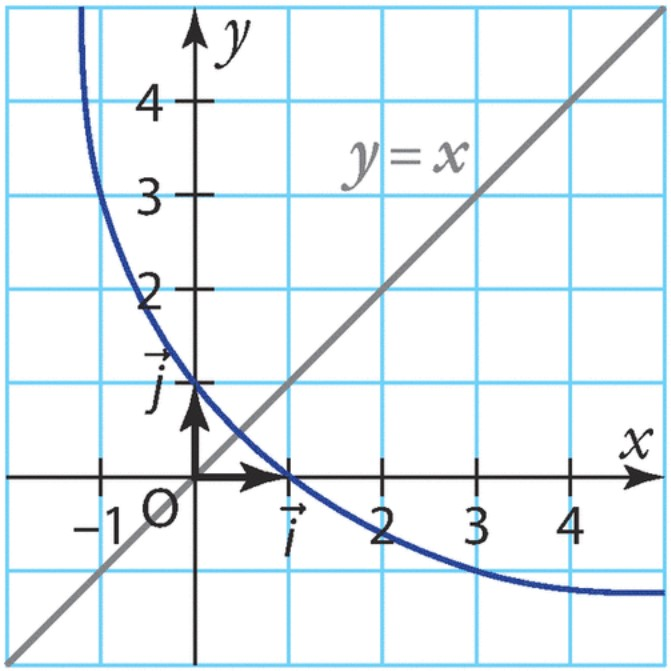
\includegraphics[width=5cm]{graphique1.jpg}}


\subsection*{Suites de références}

\exo{}
Soit $(u_n)$ une suite géométrique de raison $2$ et de premier terme $u_0=3$.
\begin{multicols}{2}
\begin{enumerate}
    \item Calculer $u_1$.
    \item Calculer $u_4$.
\end{enumerate}
\end{multicols}

\exo{}
Soit $(v_n)$ une suite aritmétique de raison $-5$ et de premier terme $v_1=4$.
\begin{multicols}{2}
\begin{enumerate}
    \item Calculer $v_2$.
    \item Calculer $v_{11}$.
\end{enumerate}
\end{multicols}

\exo{}
Soit $(w_n)$ une suite géométrique de raison $q>0$, telle que $\quad w_4=3\quad$ et $\quad w_6=48$.\\
Déterminer la valeur de $q$.

\exo{}
Soit $(t_n)$ une suite arithmétique de raison $r$ telle que $\quad t_4=3\quad$ et $\quad t_7=18$.\\
Déterminer la valeur de $r$.

\exo{}
Un contrat d'entretien d'une piscine prévoit un versement de 200 € la première année, puis des versements annuels qui augmentent de 2 \% par an.\\
Quelle somme totale aura versé le propriétaire de la piscine au bout de 15 ans ?

\exo{}
Un cycliste qui s'entraîne pour le Tour de Bretagne parcourt 100 km lors de la première semaine de son entraînement, puis il augmente chaque semaine la distance parcourue de 20 km.\\
Quelle distance aura-t-il parcourue au bout de ses 20 semaines d'entraînement ?

\exo{}
Le nombre de noyaux d'un échantillon de 500 noyaux d'iode 131 diminue chaque jour de 8,3 \%.\\
Au bout de combien de jours ce nombre aura-t-il diminué de moitié ?

\subsection*{Limite d'une suite}

\exo{}
Pour chacune des suites représentées ci-dessous, dire quelle semble être sa limite éventuelle.
\begin{multicols}{4}
    \begin{enumerate}
        \item $\ $\\
        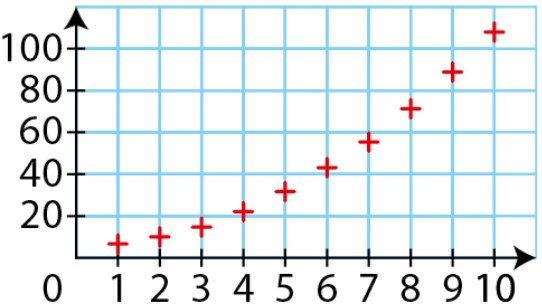
\includegraphics[width=3.5cm]{graphique_a.jpg}
        \item $\ $\\
        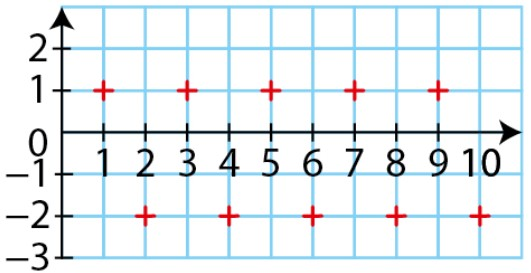
\includegraphics[width=3.5cm]{graphique_b.jpg}
        \item $\ $\\
        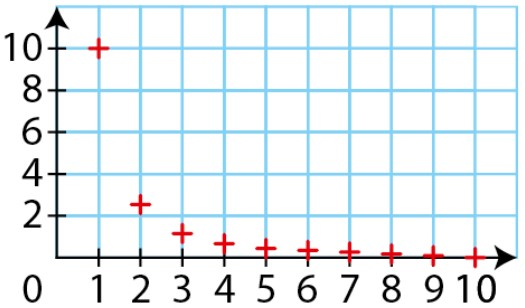
\includegraphics[width=3.5cm]{graphique_c.jpg}
        \item $\ $\\
        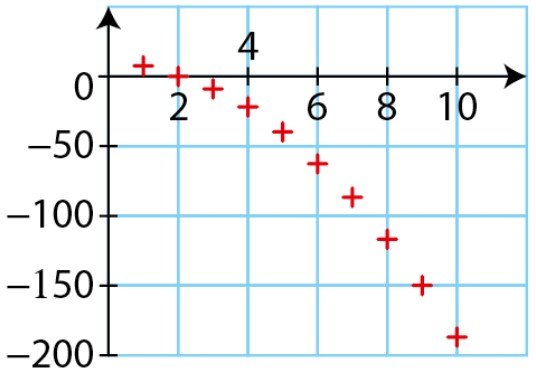
\includegraphics[width=3.5cm]{graphique_d.jpg}
    \end{enumerate}
\end{multicols}

\exo{ \faCalculator}
Dans chaque cas, à l'aide de la calculatrice, conjecturer la limite éventuelle des suites définie sur $\N$ par :
\begin{multicols}{4}
    \begin{enumerate}
        \item $u_n=-2n+3$
        \item $v_n=0,5 n^2$
        \item $w_n=1+\dfrac{1}{n+1}$
        \item $t_n=(-3)^n$
    \end{enumerate}
\end{multicols}


\exo{ \faPython}
\begin{minipage}{0.7\linewidth}
    $(u_n)$ est la suite définie sur $\N$ par :
    $$\left\{
		\begin{array}{llll}
			u_0 & = & 0 & \\
			u_{n+1} & = & 4u_n+3 & \text{pour tout } n\in\N\\
		\end{array}
    \right. $$
    Voici une fonction \mintinline{python}{seuil} ci-contre, écrite en langage Python. 
    \begin{enumerate}
        \item Quel est le rôle de cette fonction \mintinline{python}{seuil} ?
        \item Saisir et exécuter ce programme pour :
        \begin{multicols}{3}
            \begin{enumerate}[label=\textbullet]
                \item $m=1000$
                \item $m=100\ 000$
                \item $m=10^{10}$
            \end{enumerate}
        \end{multicols}
        
        \item Conjecturer la limite de la suite $(u_n)$.
    \end{enumerate}
\end{minipage}
\begin{minipage}{0.3\linewidth}
    \begin{pyc}
        \begin{minted}{python}
def seuil(m) :
    n = 0
    c = 0
    while c < m :
        c = 4*c+3
        n = n+1
    return n
        \end{minted}
    \end{pyc}
\end{minipage}
    

\exo{ Approximation de $\sqrt{2}$ par la méthode de Héron}
\textit{On attribue à Hippase de Métaponte (500 av. J.-C.) la découverte de l'irrationnalité de $\sqrt{2}$. Héron d'Alexandrie aurait établi une méthode pour approcher ce nombre (et plus largement la racine carrée de n'importe quel entier).}\\[.5em]
Calculer $\sqrt{2}$ revient à construire un carré dont l'aire est 2.\\[.5em]
Pour $x>0$, si on construit un rectangle de premier côté $x$ et d'aire 2, le deuxième côté aura pour longueur $\dfrac{2}{x}$, car $x\times \dfrac{2}{x}=2$.\\[.5em]
\faLightbulb \hspace*{.3cm} On construit ensuite un deuxième rectangle d'aire 2 dont le premier côté a pour longueur la moyenne des côtés du rectangle précédent, soit $\dfrac{1}{2}\left(x+\dfrac{2}{x}\right)$. On réitère ce processus aussi longtemps que l'on veut ; on peut démontrer que le rectangle ainsi construit s'approche de plus en plus d'un carré de côté $\sqrt{2}$.
\begin{enumerate}
    \item Montrer que si $x_0$ est une valeur approchée par excès de $\sqrt{2}$, alors $\dfrac{2}{x}$ est une valeur approchée par défaut de $\sqrt{2}$, et inversement.
    \item On choisit $x_0=2$ comme première valeur approché de $\sqrt{2}$. On étudie la suite $(x_n)$ définie sur $\N$ par : 
    $$\left\{
		\begin{array}{llll}
			x_0 & = & 2 & \\
			x_{n+1} & = & \dfrac{1}{2}\left(x_n+\dfrac{2}{x_n}\right) & \text{pour tout } n\in\N\\
		\end{array}
    \right. $$
    \begin{minipage}{11cm}
        \begin{enumalph}
            \item Représenter graphiquement la fonction $f$ telle que\\ $x_{n+1}=f(x_n)$, ainsi que les premiers termes de la suite $(x_n)$.
            \item Conjecturer le sens de variation et la convergence de la suite $(x_n)$.
            \item Compléter la fonction \mintinline{python}{heron} ci-contre de paramètre \mintinline{python}{p} pour qu'elle renvoie un encadrement d'amplitude $10^{-p}$ de $\sqrt{2}$.
            \item Donner un encadrement d'amplitude $10^{-15}$ de $\sqrt{2}$.
        \end{enumalph}
    \end{minipage} \hspace*{.3cm}
    \begin{minipage}{5.5cm}
        \begin{pyc}
            \begin{minted}{python}
                def heron(p) :
                    x = 2
                    y = ...
                    while x-y > ... :
                        x = ...
                        y = ...
                    return(y,x)
            \end{minted}
        \end{pyc}
    \end{minipage}
\end{enumerate}

\exo{}
Calculer la limite de chacune des suites définies sur $\N$ par :
\begin{multicols}{2}
    \begin{enumerate}
        \item $u_n=-n^2-6n+15$
        \item $v_n=\dfrac{8}{-3n+1}$
        \item $w_n=\left(\dfrac{5}{n^2}+4\right)\left(3-\sqrt{n}\right)$
        \item $t_n=\dfrac{5n+3}{n}$
    \end{enumerate}
\end{multicols}


\exo{}
Soit $(u_n)$ la suite définie sur $\N$ par : $\quad u_n=n^2-4n+1$.
\begin{enumerate}
    \item Expliquer pourquoi on ne peut pas déterminer la limite de $(u_n)$ avec les propriétés des limites.
    \item Montrer que, pour tout entier naturel $n$ non nul : $\quad u_n=n^2 \left(1-\dfrac{4}{n}+\dfrac{1}{n^2}\right)$.
    \item En déduire la limite de $(u_n)$.
\end{enumerate}

\exo{}
Soit $(v_n)$ la suite définie sur $\N$ par : $\quad v_n=\dfrac{2n+1}{3n+2}$.
\begin{enumerate}
    \item Expliquer pourquoi on ne peut pas déterminer la limite de $(v_n)$ avec les propriétés des limites.
    \item Montrer que, pour tout entier naturel $n$ non nul : $\quad v_n=\dfrac{n\left(2+\dfrac{1}{n}\right)}{n\left(3+\dfrac{2}{n}\right)}$.
    \item En déduire la limite de $(v_n)$.
\end{enumerate}

\subsection*{Comparaisons de limites}

\exo{}
Déterminer la limite de chacune des suites dont le terme général est donné ci-dessous.
\begin{multicols}{2}
    \begin{enumerate}
        \item $u_n=n^3+(-1)^n\quad$ pour $n\in\N$
        \item $v_n=\dfrac{2+(-1)^n}{n}\quad$ pour $n\in\N^*$
        \item $w_n=\sqrt{n^2+3n+5}\quad$ pour $n\in\N$
        \item $t_n=\dfrac{4n+(-1)^n}{n}\quad$ pour $n\in\N^*$
    \end{enumerate}
\end{multicols}

\exo{}
Soit $(u_n)$ la suite définie sur $\N$ par : $\quad u_n=n^2-3n+1$.
\begin{enumerate}
    \item Montrer que pour tout $n\in\N, \quad u_n>n(n-3)$.
    \item En déduire la limite de la suite $(u_n)$.
\end{enumerate}

\exo{}
Soit $(v_n)$ la suite définie sur $\N$ par : $\quad v_n=1+\dfrac{(-1)^n}{n+1}$.
\begin{enumerate}
    \item Donner un encadrement de $v_n$ pour $n\in\N$.
    \item En déduire la limite de la suite $(v_n)$.
\end{enumerate}


\exo{}
Soit $(w_n)$ la suite définie sur $\N$ par : $\quad w_n=\dfrac{n^2}{n+1}$.
\begin{enumerate}
    \item Montrer que pour tout $n\in\N, \quad w_n>n-1$.
    \item En déduire la limite de la suite $(w_n)$.
\end{enumerate}

\subsection*{Limites et suites géométriques}

\exo{}
Dans chaque cas, préciser la raison de la suite géométrique définie sur $\N$ et donner sa limite.
\begin{enumerate}
    \item $u_0=-1\quad$ et, pour tout $n\in\N, \quad u_{n+1}=2,5\ u_n$.
    \item $v_0=1\quad$ et, pour tout $n\in\N, \quad v_{n+1}=1,5\ v_n$.
    \item $w_0=1\quad$ et, pour tout $n\in\N, \quad w_{n+1}=0,5\ w_n$.
    \item $t_0=-1\quad$ et, pour tout $n\in\N, \quad t_{n+1}=\dfrac{1}{4}\ t_n$.
\end{enumerate}

\exo{}
On a représenté quatre suites géométriques $(u_n), (v_n), (w_n)$ et $(t_n)$ dans un repère.\\

\dleft{6cm}{
    \begin{enumerate}
        \item Associer chaque graphique à la suite géométrique définie sur $\N$ qui lui correspond.
        \begin{enumerate}[label=\textbullet]
            \item $u_n=3\times 1,1^n$
            \item $v_n=-2\times 2,1^n$
            \item $w_n=2\times 0,8^n$
            \item $t_n=-3\times 1^n$
        \end{enumerate}
        \item En déduire, en justifiant, la limite de chaque suite.
    \end{enumerate}
}
{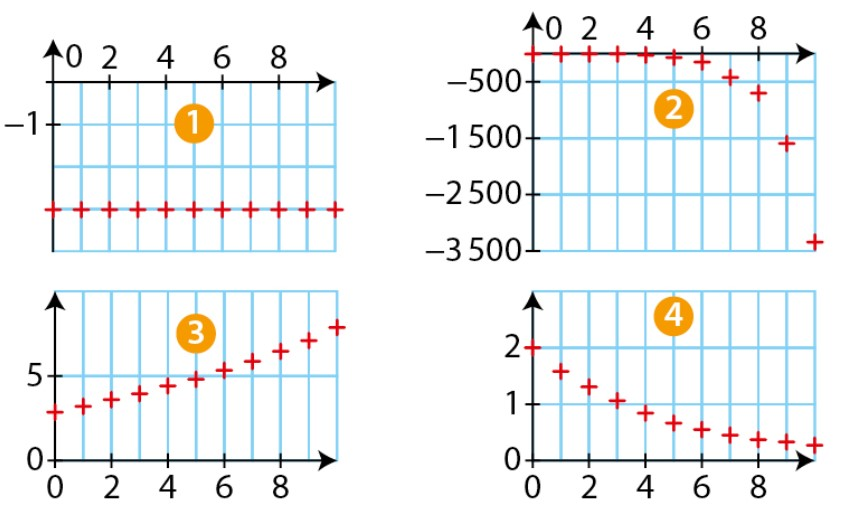
\includegraphics[width=10cm]{graphique2.jpg}}



\exo{}
Dans chaque cas, déterminer en justifiant la limite de la suite définie sur $\N$ par :
\begin{multicols}{4}
    \begin{enumerate}
        \item $u_n=7\left(2-0,2^n\right)$
        \item $v_n=\dfrac{1+0,7^n}{2^n}$
        \item $w_n=5^n-\left(\dfrac{1}{4}\right)^n$
        \item $t_n=\dfrac{3n+5^n}{1-\dfrac{1}{n^2}}$
    \end{enumerate}
\end{multicols}

\exo{}
Déterminer la limite de la suite $(S_n)$ définie sur $\N$ par $\quad S_n=1+\dfrac{1}{4}+\left(\dfrac{1}{4}\right)^2+...+\left(\dfrac{1}{4}\right)^n$.


\exo{}
$(u_n)$ est la suite géométrique de raison $0,8$ telle que $u_0=3$.\\
Pour tout $n\in\N$, on note $\quad S_n=u_0+u_1+...+u_n$.
\begin{enumerate}
    \item Exprimer $S_n$ en fonction de $n$.
    \item Donner la limite de la suite $(S_n)$.
\end{enumerate}

\exo{ \faCalculator \hspace*{.3cm} Propagation d'une rumeur}
Dans un lycée de 800 élèves, un élève dévoile un secret à deux de ses camarades, puis se tait. Le lendemain, chaque camarade ayant appris le secret le dit à deux élèves qui ne le connaissent pas, puis se tait. La même règle est appliquée les jours suivants.\\
Déterminer le nombre de jours nécessaires pour que tous les élèves du lycée connaissent la rumeur.

\exo{}
\dleft{12cm}{
    \begin{enumerate}
        \item En traçant la diagonale d'un carré de côté 1, on obtient un triangle rectangle que l'on colorie, comme sur la figure ci-contre.\\
        Calculer l'aire de ce triangle.
        \item On construit de la même manière un triangle rectangle que l'on colorie dans le quart du carré en haut à droite, et ainsi de suite... On obtient un ensemble de $n$ triangles colorés dont l'aire totale est notés $A_n$, pour $n$ entier supérieur ou égal à 1.\\
        Quelle est la limite de la suite $(A_n)$ ?
    \end{enumerate}
    
}
{
    \begin{tikzpicture}[scale=.5]
        %\clip(0,0) rectangle (8,8);
        \draw[thick,UGLiOrange, fill=UGLiOrange!50] (0,0) -- (8,0)  -- (0,8) -- (0,0);
        \draw[thick,UGLiOrange, fill=UGLiOrange!50] (4,4) -- (8,4)  -- (4,8) -- (4,4);
        \draw[thick,UGLiOrange, fill=UGLiOrange!50] (6,6) -- (8,6)  -- (6,8) -- (6,6);
        \draw[thick,UGLiOrange, fill=UGLiOrange!50] (7,7) -- (8,7)  -- (7,8) -- (7,7);
        \draw[thick,UGLiOrange, fill=UGLiOrange!50] (7.5,7.5) -- (8,7.5)  -- (7.5,8) -- (7.5,7.5);
        \draw[thick,UGLiOrange] (8,0) -- (8,8) -- (0,8) ;
    \end{tikzpicture}
}

\exo{ \faPython \hspace*{.3cm} Évolution d'une population de bactéries}
Un échantillon de 100 mL d'eau contient 50 000 bactéries pathogènes, rendant un plan d'eau impropre à la baignade. En temps normal, le nombre de bactéries diminue de 10 \% chaque jour.
\begin{enumerate}
    \item \begin{enumalph}
        \item Modéliser l'évolution du nombre quotidien de bactéries à l'aide d'une suite dont on précisera le terme général.
        \item Quelle est la limite de cette suite ?
        \item La baignade sera à nouveau autorisée lorsqu'il n'y aura pas plus de 100 bactéries dans un échantillon de 100 mL.\\
        \faCalculator \hspace*{.3cm} Déterminer le nombre de jours nécessaires pour que la baignade soit à nouveau autorisée.
    \end{enumalph}
    
    \begin{minipage}{11cm}
        \item \faPython \hspace*{.3cm} On veut écrire en langage Python une fonction \mintinline{python}{seuil} pour répondre à la question précédente.
        \begin{enumalph}
            \item Compléter le script.
            \item Utiliser la fonction \mintinline{python}{seuil} pour retrouver la réponse à la question \textbf{1.c}. 
        \end{enumalph}
    \end{minipage}
    \begin{minipage}{4.5cm}
        \begin{pyc}
            \begin{minted}{python}
                def seuil(m) :
                    n = 0
                    c = 50000
                    while c>m :
                        c = ...
                        n = ...
                    return n
            \end{minted}
        \end{pyc}
    \end{minipage}
\end{enumerate}


\exo{ \faSplotch}
Déterminer la limite de la suite définie sur $\N$ par : $\quad u_n = \dfrac{5^n-4^n}{5^{n+1}-4^{n+1}}$

\subsection*{Suites arithmético-géométriques}

\exo{ Évolution d'une population de macareux moines}
\picleftc{0.25}{puffins.jpg}{Image : Pixabay}{
    Sur une petite île de l'Atlantique Nord, on a observé l'évolution d'une population de macareux moines depuis plusieurs années.\\
    Il y avait 600 macareux moines sur l'île au 1$^{\text{er}}$ juin 2020.\\
    On note $u_n$ l'effectif de cette population au 1$^{\text{er}}$ juin 2020$+n$.\\ Les observations permettent de modéliser cette évolution par la relation $\quad u_{n+1}=0,7\ u_n+30\quad$ pour tout entier naturel $n$.
}
\begin{enumerate}
    \item Montrer que cette relation de récurrence est vérifiée par la suite constante $(c_n)$ telle que pour tout $n\in\N, \ c_n=100$.
    \item Soit $(v_n)$ la suite définie sur $\N$ par $v_n=u_n-c_n$.
    \begin{enumalph}
        \item Montrer que $(v_n)$ est une suite géométrique.
        \item Montrer que $v_0=500$ et en déduire l'expression de $v_n$ en fonction de $n$.
        \item En déduire que pour tout $n\in\N, \quad u_n=500\times 0,7^n+100$.
    \end{enumalph}
    \item Estimer avec ce modèle la population de macareux moines au 1$^{\text{er}}$ juin 2025 sur cette île.
\end{enumerate}

\exo{}
Soit $(u_n)$ la suite définie sur $\N$ par : 
$\quad \left\{
    \begin{array}{llll}
        u_0 & = & -2 & \\
        u_{n+1} & = & 5u_n-12 & \text{pour tout } n\in\N\\
    \end{array}
\right. $
\begin{enumerate}
    \item Déterminer la suite constante $(c_n)$ qui vérifie la relation de récurrence $\quad c_{n+1}=5c_n-12\quad$ pour tout $n\in\N$.
    \item En déduire le terme général de la suite $(u_n)$.
\end{enumerate}

\exo{}
On considère la suite $(v_n)$ définie sur $\N$ par $\quad v_0=8\quad$ et, pour tout $n\in\N, \quad v_{n+1}=0,1v_n+9$.
\begin{enumerate}
    \item Déterminer le terme général de la suite $(v_n)$.
    \item En déduire la limite de $(v_n)$.
\end{enumerate}

\exo{ \faPython \hspace*{.3cm}}
Tous les ans, au mois de septembre, une association prélève 8,5 tonnes d'algues sur les plages d'une commune.\\
Au 1$^{\text{er}}$ septembre 2024, il y avait 230 tonnes d'algues sur ces plages.\\
Tous les ans, entre le 1$^{\text{er}}$ octobre et le 1$^{\text{er}}$ septembre suivant, la quantité d'algues sur ces plages augmente de 4 \%. On note $u_n$ la quantité d'algues (en tonnes) présente sur les plages au 1$^{\text{er}}$ septembre de l'année 2024$+n$.
\begin{enumerate}
    \item Montrer que pour tout entier naturel $n, \quad u_{n+1}=1,04\ u_n-8,84$.
    \item Déterminer l'expression de $u_n$ en fonction de $n$.
    \item La quantité d'algues sur ces plages dépassera-t-elle un jour 250 tonnes ?
    \item Une usine de transformation d'algues en plastique prévoit de s'installer dans la commune en septembre 2025. Elle solicite l'association pour lui fournir chaque année 10 \% d'algues de plus que l'année précédente.\\
    \begin{minipage}{8cm}
        \begin{pyc}
            \begin{minted}{python}
                def algues(...) :
                    plage = 230
                    ramasse = 8.5
                    for i in range(...) :
                        plage = ...
                        ramasse = ...
                    return(plage,ramasse)
            \end{minted}
        \end{pyc}
    \end{minipage}
    \begin{minipage}{8cm}
        Compléter le programme ci-contre pour que l'appel \mintinline{python}{algues(n)} renvoie la quantité d'algues sur les plages et la quantité d'algues ramassées en 2025$+n$.\\

        Quelle quantité d'algues serait ainsi présente sur la plage dans 10 ans ? Dans 20 ans ?\\
        Qu'en pensez-vous ?
    \end{minipage}
\end{enumerate}

%\subsection*{Suites croisées}


\subsection*{Prolongements}


\exo{ \faSplotch}
Soit la suite $(u_n)$ défine $\N$ par : 
$\quad \left\{
    \begin{array}{llll}
        u_0 & = & 1 & \\
        u_{n+1} & = & \dfrac{u_n}{2u_n+3} & \text{pour tout } n\in\N\\
    \end{array}
\right. $\\[.5em]
On admet que pour tout $n\in\N, u_n$ ne s'annule pas.\\[.5em]
En utilisant la suite de terme général $v_n=\dfrac{1}{u_n}$, déterminer l'expression de $u_n$ en fonction de $n$.


\newpage
\exo{Approximation de $\pi$ par la méthode d'Archimède}
\dleft{14cm}{
    \textcolor{UGLiBlue}{
    Archimède de Syracuse (287 av. J.-C - 212 av. J.-C.) est un grand scientifique grec de Sicile de l'Antiquité : physicien, astronome, mathématicien et ingénieur. Selon la légende, il aurait compris le principe que nous appelons aujourd'hui « poussée d'Archimède » dans son bain et aurait couru nu à travers les rues de la ville en criant \textit{« Eurêka ! »} (« J'ai trouvé ! »).
}
}{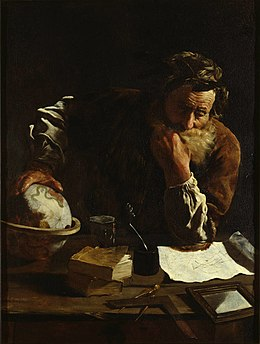
\includegraphics[width=2.5cm]{Archimede_Domenico_Fetti.jpg}}

\begin{enumerate}
    \item Rappeler le périmètre d'un cercle de rayon 1.
\end{enumerate}
\dleft{6cm}{
    La méthode d'Archimède consiste à encadrer le périmètre d'un cercle de rayon 1 par les périmètres de polygones réguliers inscrits et circonscrits ayant de plus en plus de côtés.\\
}
{
    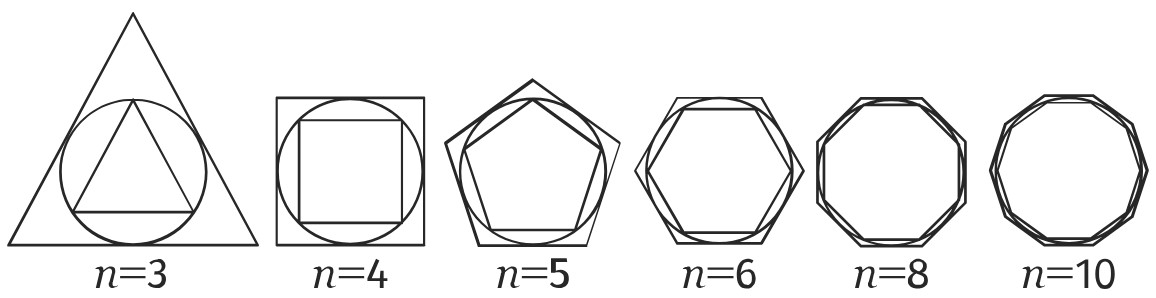
\includegraphics[width=10cm]{polygones.jpg}
}
On note $P_n$ le périmètre du polygone régulier intérieur à $n$ côtés et $P'_n$ le périmètre du polygone régulier extérieur à $n$ côtés.

\dleft{10cm}{
    \begin{enumerate}[label=\textbf{2.}]
        \item  \textbf{Étude du cas $n=6$ :}
    \end{enumerate}
    \begin{enumalph}
        \item À l'aide de la figure, justifier que $P_6=6$.
        \item Calculer $\tan(30°)$.
        \item Utiliser le résultat précédent pour démontrer que\\ $P'_6=4\sqrt{3}$.
        \item En déduire une première approximation de $\pi$.
    \end{enumalph}
}
{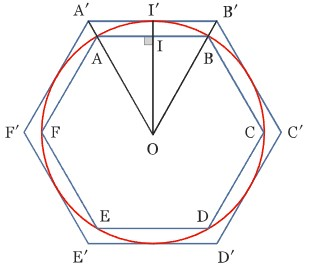
\includegraphics[width=6cm]{p6.jpg}}
\begin{enumerate}[label=\textbf{3.}]
    \item  Démontrer que pour tout $n\in\N, \quad P_n=2n\sin\left(\dfrac{180°}{n}\right)\quad$ et $\quad P'_n=2n\tan\left(\dfrac{180°}{n}\right)$.
\end{enumerate}
\begin{enumerate}[label=\textbf{4.}]
    \item  \textbf{Utilisation d'un algorithme :}
\end{enumerate}
On souhaite créer un programme permettant de calculer une approximation de $\pi$ avec une précision $p$ donnée.
\begin{enumalph}
    \item Compléter la première partie de l'activité Capytale \textbf{ef30-3390279}. 
    \item Pour obtenir une approximation de $\pi$ à $10^{-3}$ près, combien de côtés doivent avoir les polygones réguliers à utiliser ?
\end{enumalph}


\end{document}